\documentclass[11pt]{beamer}
\mode<presentation>
\usetheme{metropolis}
\usecolortheme[named=black]{structure}
\usefonttheme{professionalfonts}

\usepackage{appendixnumberbeamer}

\usepackage[utf8]{inputenc}
\usepackage[spanish]{babel}
\usepackage{geometry}
  \geometry{
    left=10mm,
    right=10mm,
    top=10mm,
    bottom=10mm,
  }
\usepackage{graphicx}
\usepackage{multicol}
\usepackage{algorithm,algorithmic}


\title{Desarrollo y control de una gimbal de dos grados de libertad mediante visión artificial para el seguimiento
de objetivos}
\author{Marco Antonio Aguilar Gallardo}
\institute{Universidad Aeronáutica en Querétaro}
\date{\today}

\begin{document}
  \frame{\titlepage}

  \begin{frame}
    \frametitle{Tabla de contenido}
    \tableofcontents
  \end{frame}

% !=============== INTRODUCCION ===============
  \section{Introducción}
  %* --Nueva diapositiva
  \begin{frame}[t]
    \frametitle{Introducción}
    \begin{itemize}
    \item La gimbal ha estado presente desde el siglo 3 antes de cristo.
    \item Utilizada en amplios sectores como el maritimo, aeronautico y entretenimiento.
    \end{itemize}
    \begin{figure}[h]
      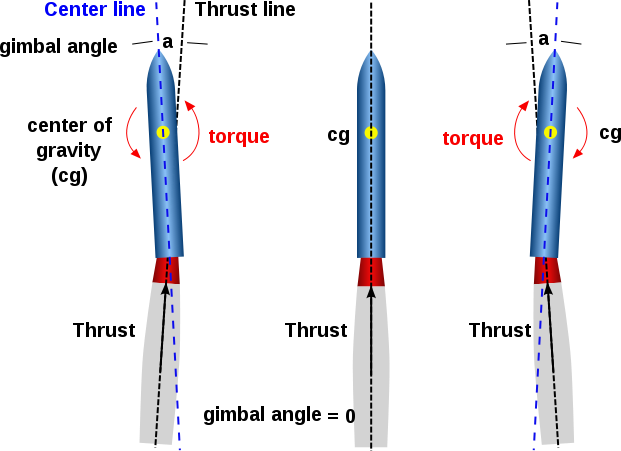
\includegraphics[height=3cm, keepaspectratio]{images/rocket.png}
      \caption{Gimbal para estabilizar motores}
      \label{fig:rocket}
    \end{figure}
  \end{frame}
  %* --Nueva diapositiva
  \begin{frame}
    \frametitle{Introducción}
    \begin{multicols*}{2}
      \begin{itemize}
        \item 3 grados de libertad
        \item Acelerometro
        \item Giroscopio
      \end{itemize}
      \begin{figure}[h]
        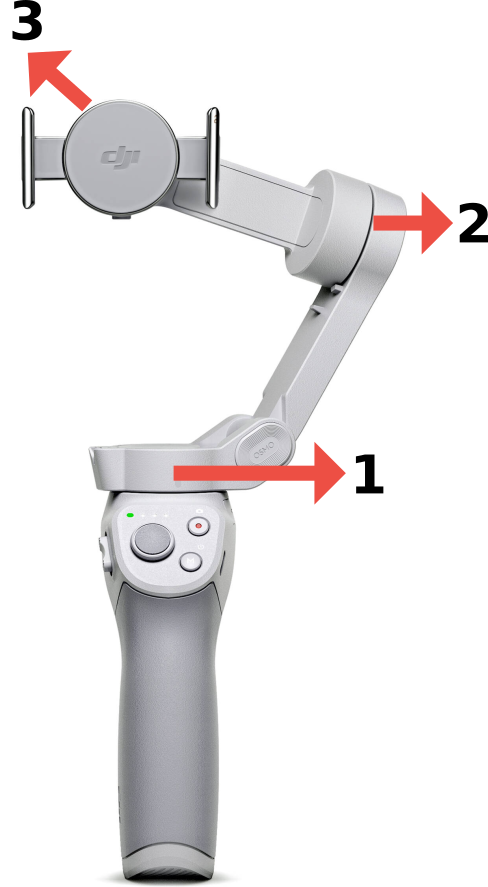
\includegraphics[height=5cm, keepaspectratio]{images/dji.png}
        \caption{Gimal DJI, tomada de dji.com}
        \label{dji}
      \end{figure}
    \end{multicols*}
  \end{frame}
  %* --Nueva diapositiva
  \begin{frame}
    \frametitle{Objetivo}
    Diseñar, instrumentar y controlar un dispositivo gimbal que sea capaz de
    seguir un objeto a través de visión artificial para implementarse en un UAV
    de categoría pequeña a velocidad baja.
  \end{frame}

% !=============== DESARROLLO ===============
  \section{Desarrollo}
  %* --Nueva diapositiva
  \begin{frame}
    \frametitle{Sistema General}
    \begin{figure}[h]
      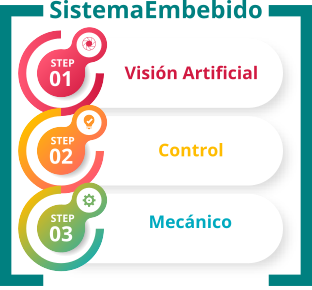
\includegraphics[height=6cm, keepaspectratio]{images/sistemas.png}
    \end{figure}
  \end{frame}
  %* --Nueva diapositiva
  \begin{frame}
    \frametitle{Visión Artificial} 
    \begin{algorithm}[H]
      \begin{algorithmic}[1]
        \STATE{Calibrar cámara}
        \STATE{Capturar frames a 60fps}
        \STATE{Publicar frames en ROS}
        \STATE{Corrección de brillo y saturación}
        \STATE{Convertir RGB a HSV}
        \STATE{Acotar el modelo HSV al color de elección}
        \STATE{Agregar filtro morfológico}
        \STATE{Obtener centroide de la figura obtenida en 7}
        \STATE{Publicar coordenadas del centroide}
      \end{algorithmic}
      \caption{Visión}
      \label{alg:seq}
      \end{algorithm}
  \end{frame}
  %* --Nueva diapositiva
  \begin{frame}
    \frametitle{Calibración de cámara}
    \begin{multicols}{2}
      \begin{figure}[h]
        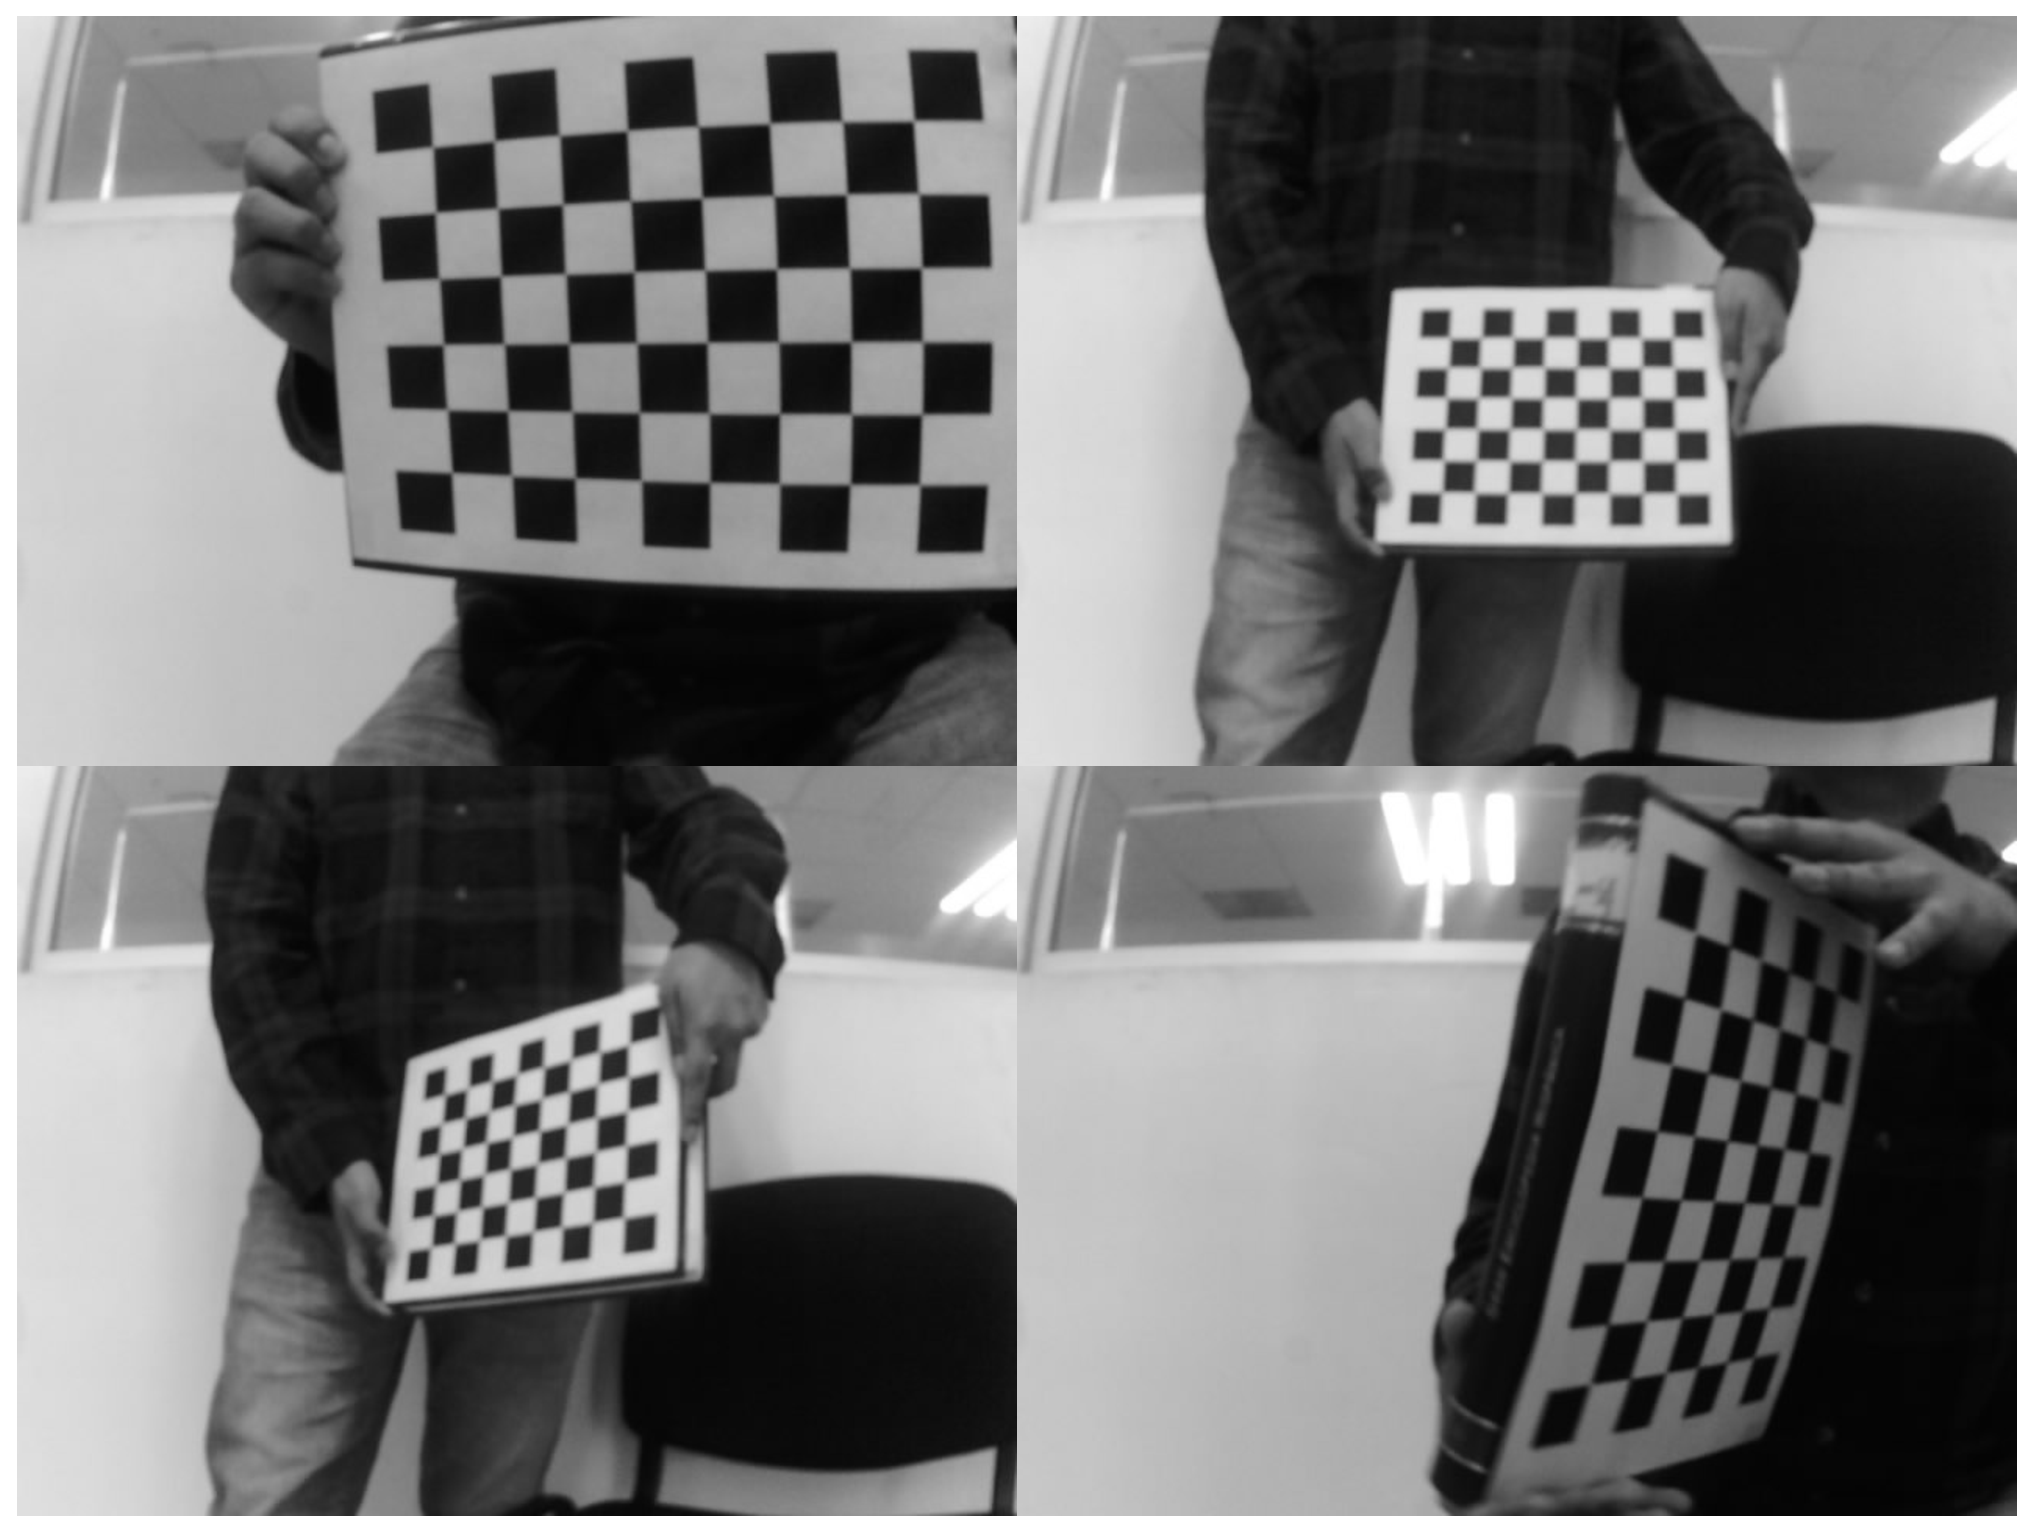
\includegraphics[width=5.2cm, keepaspectratio]{images/calibracion.eps}
        \caption{Proceso de calibración}
      \end{figure}    
      \begin{figure}[h]
        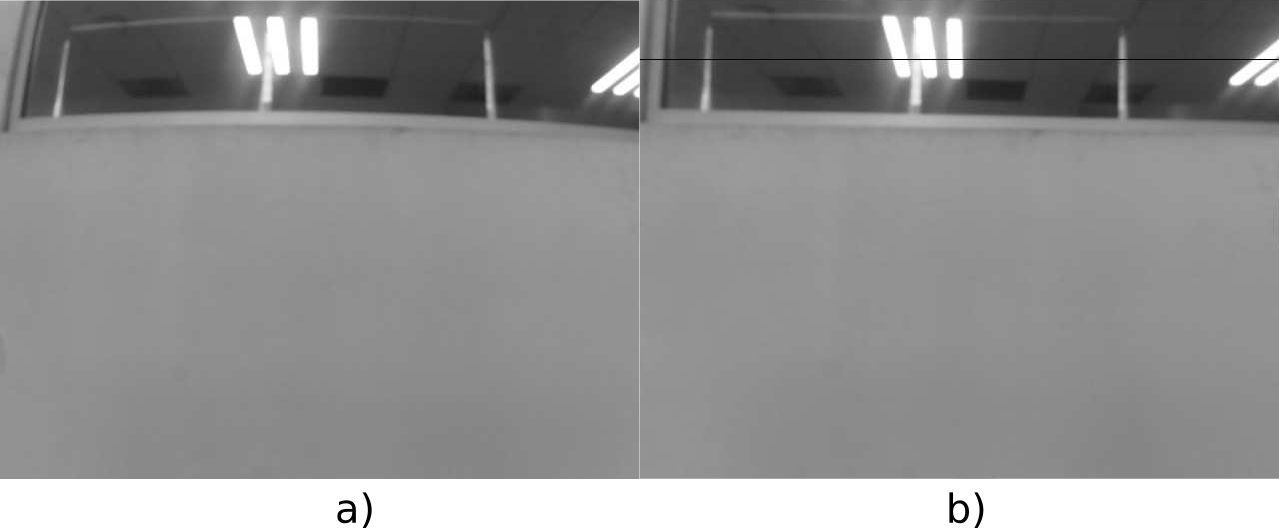
\includegraphics[width=6cm, keepaspectratio]{images/res-calibracion.png}
        \caption{Resultado}
      \end{figure}    
    \end{multicols}
  \end{frame}
  % \begin{frame}
  %   \frametitle{Calibración de cámara}
  %   \begin{figure}[h]
  %     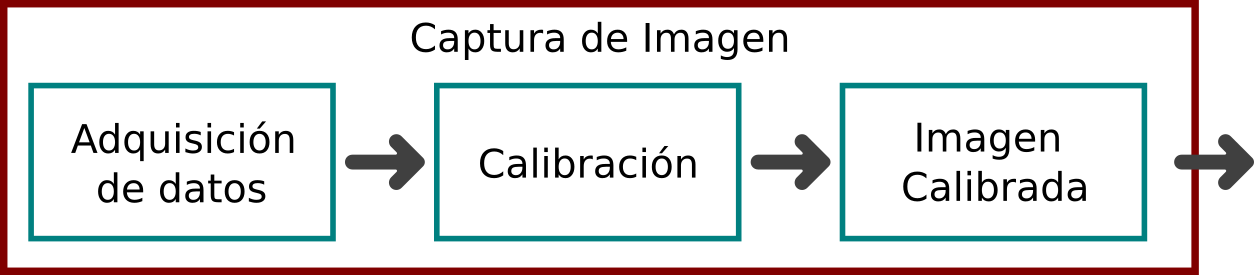
\includegraphics[width=10cm, keepaspectratio]{images/flowchart1.png}
  %   \end{figure}
  % \end{frame}
  %* --Nueva diapositiva
  \begin{frame}
    \frametitle{Espacio de Color}
    \begin{itemize}
      \item Cambio del espacio de color de RGB a HSV
    \end{itemize}
    \begin{figure}[h]
      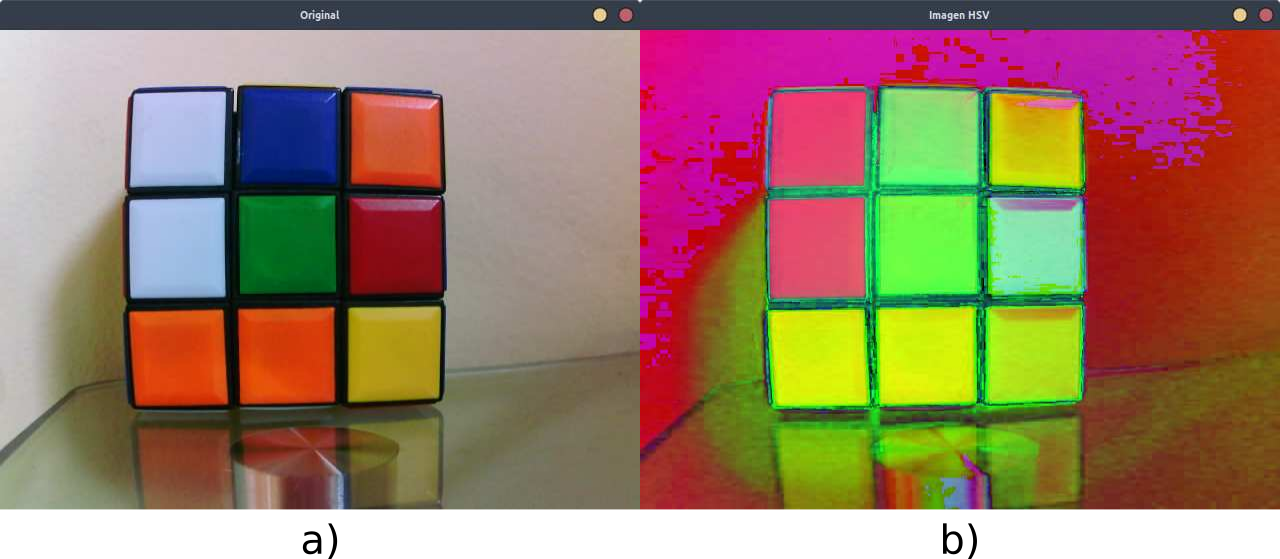
\includegraphics[width=10cm, keepaspectratio]{images/hsv.png}
    \end{figure}
  \end{frame}
  %* --Nueva diapositiva
  \begin{frame}
    \frametitle{Espacio de color}
    \begin{figure}[h]
      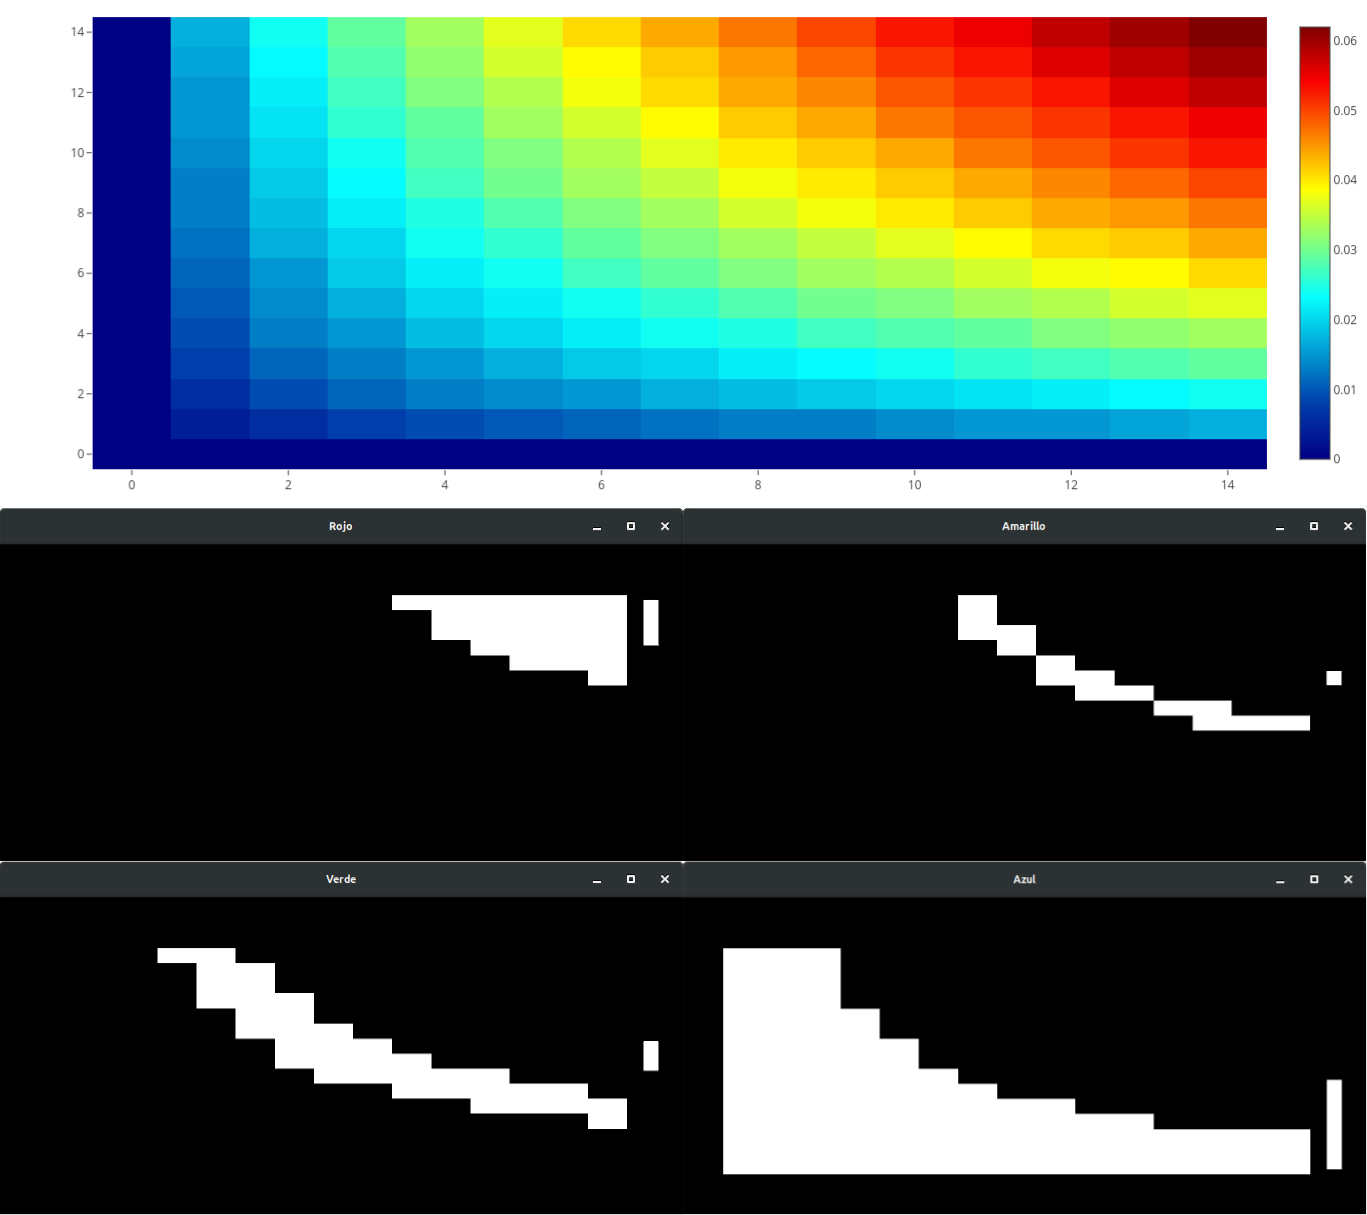
\includegraphics[height=6cm, keepaspectratio]{images/HSV.png}
      \caption{Separación de colores}
    \end{figure}
  \end{frame}
  %* --Nueva diapositiva
  \begin{frame}
    \frametitle{Espacio de color}
    \begin{table}[ht]
      \begin{center}
        \begin{tabular}[t]{lcccccc}
          \hline
                   & H$_{min}$ & H$_{max}$ & S$_{min}$ & S$_{max}$ & V$_{min}$ & V$_{max}$ \\
          \hline
          Rojo     & 0         & 10        & 100       & 255       & 100       & 255       \\
          Amarillo & 25        & 35        & 50        & 255       & 50        & 255       \\
          Verde    & 35        & 75        & 100       & 255       & 100       & 255       \\
          Azul     & 75        & 130       & 55        & 255       & 55        & 255       \\
          \hline
        \end{tabular}
        \caption{Valores para cada rango de color de la figura 5}
      \end{center}
    \end{table}
  \end{frame}
  %* --Nueva diapositiva
  \begin{frame}
    \frametitle{Espacio de color}
    \begin{figure}[h]
      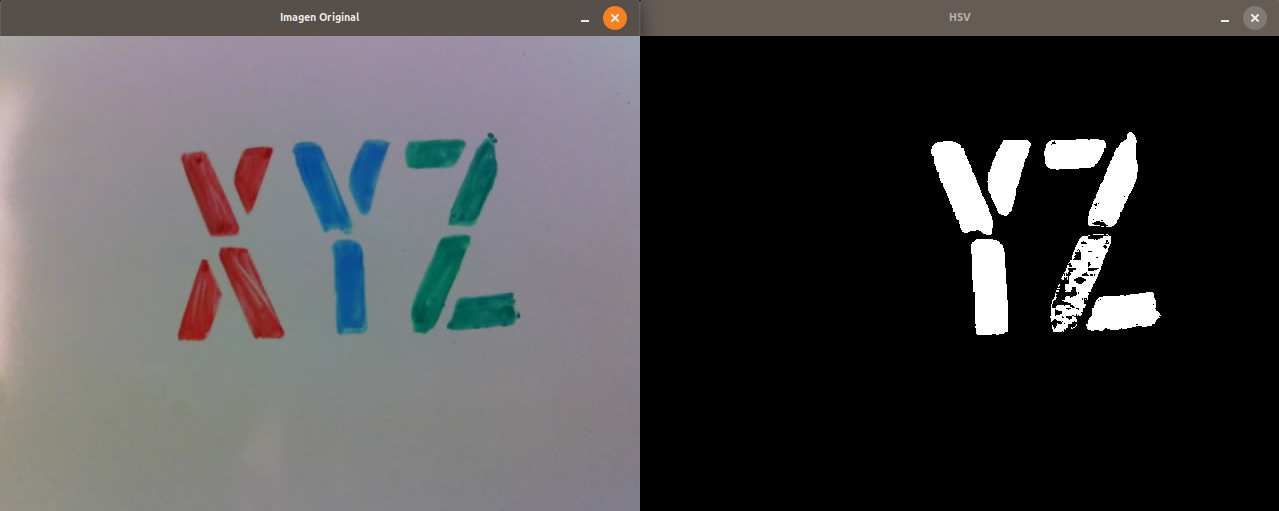
\includegraphics[height=4cm, keepaspectratio]{images/hsv-separacion.png}
      \caption{Separación de color azul}
    \end{figure}
  \end{frame}
  %* --Nueva diapositiva
  \begin{frame}
    \frametitle{Corección de brillo}
    \begin{figure}[h]
      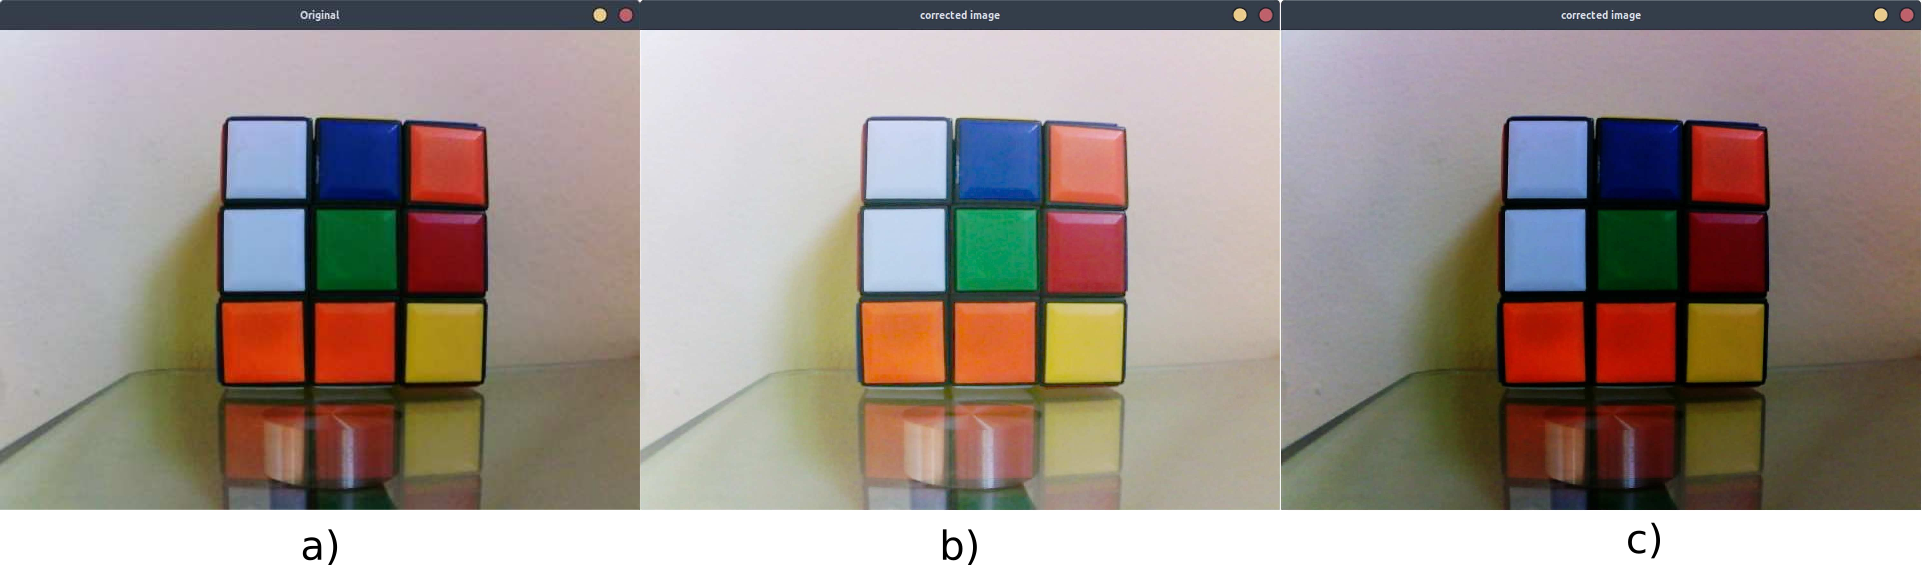
\includegraphics[width=10.5cm, keepaspectratio]{images/gamma.png}
      \caption{Correción de brillo}
    \end{figure}
  \end{frame}
  %* --Nueva diapositiva
  \begin{frame}
    \frametitle{Corección de brillo}
    \begin{figure}[h]
      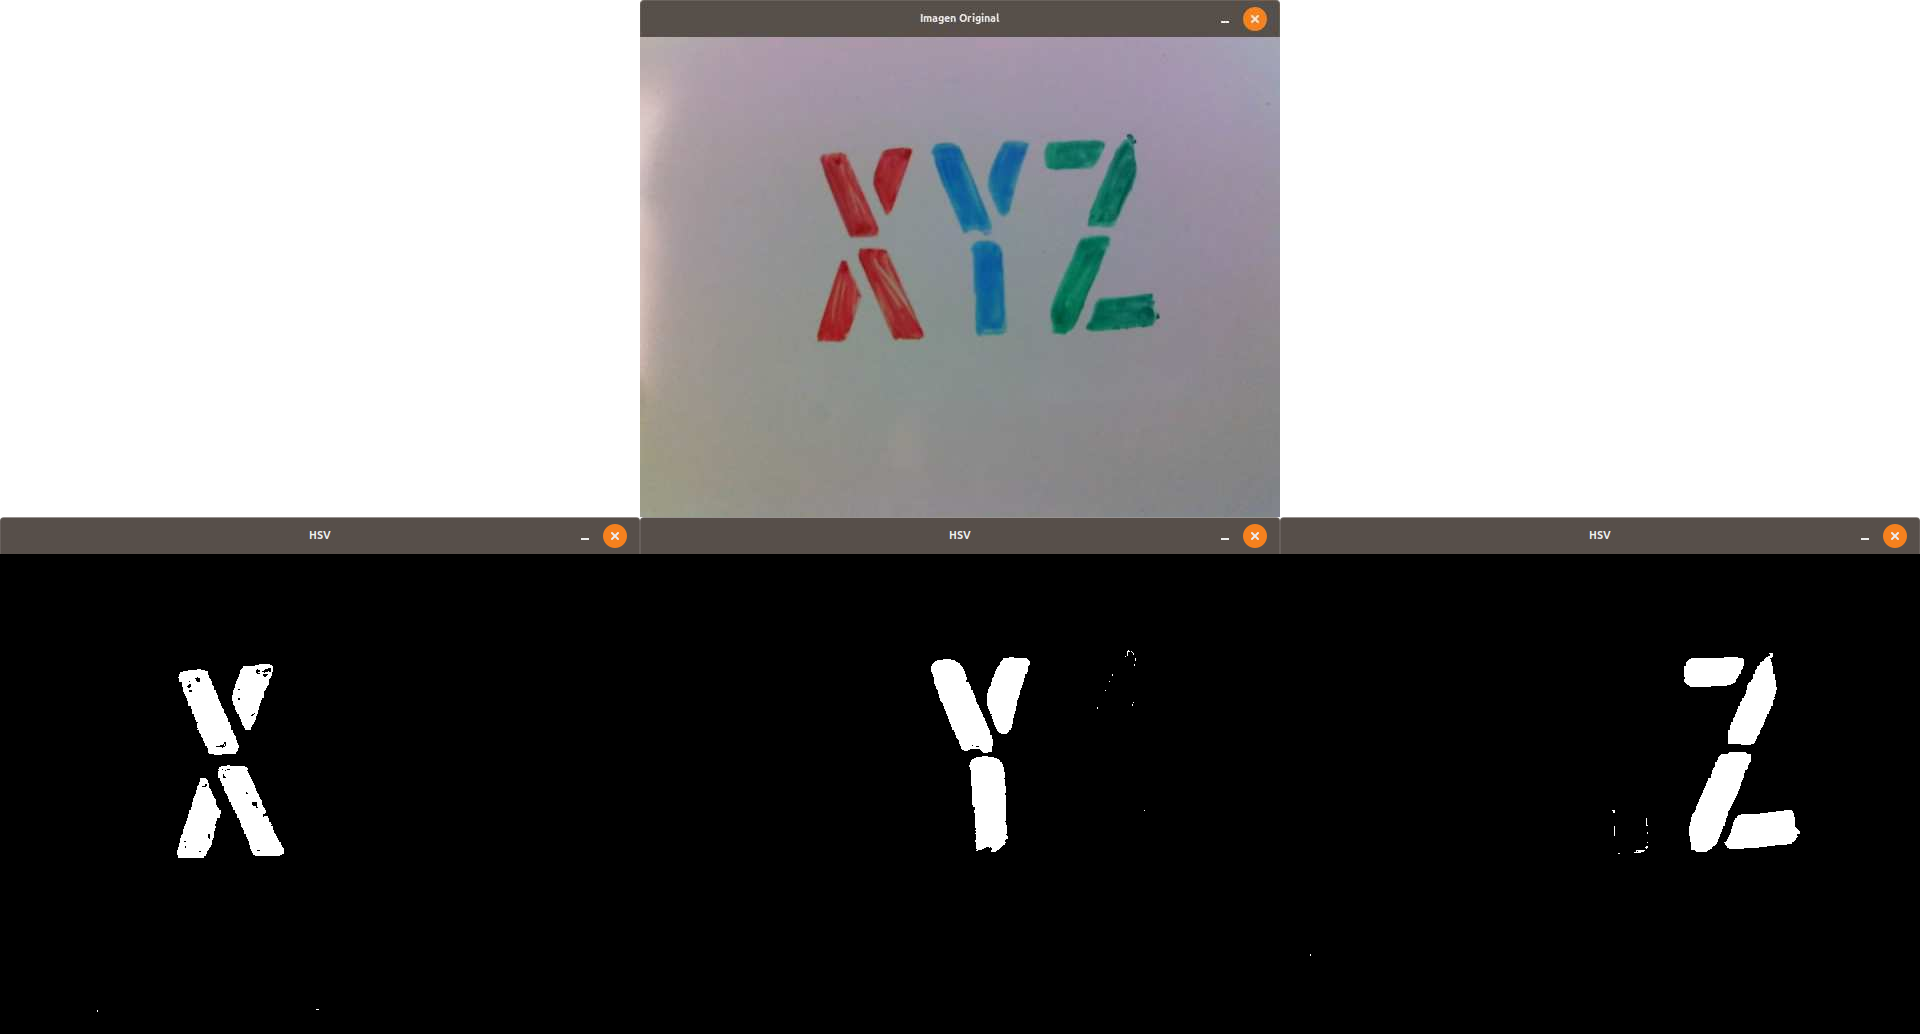
\includegraphics[width=10.5cm, keepaspectratio]{images/separacion-colores.png}
      \caption{Separación de colores después de corregir brillo}
    \end{figure}
  \end{frame}
  % %* --Nueva diapositiva
  % \begin{frame}
  %   \frametitle{Corección de brillo}
  %   \begin{figure}[h]
  %     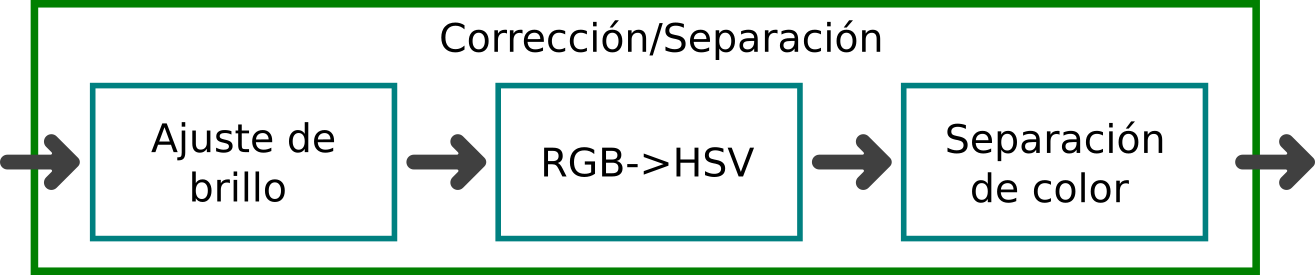
\includegraphics[width=10.5cm, keepaspectratio]{images/flowchart2.png}
  %   \end{figure}
  % \end{frame}
  %* --Nueva diapositiva
  \begin{frame}
    \frametitle{Filtro}
    \begin{figure}[h]
      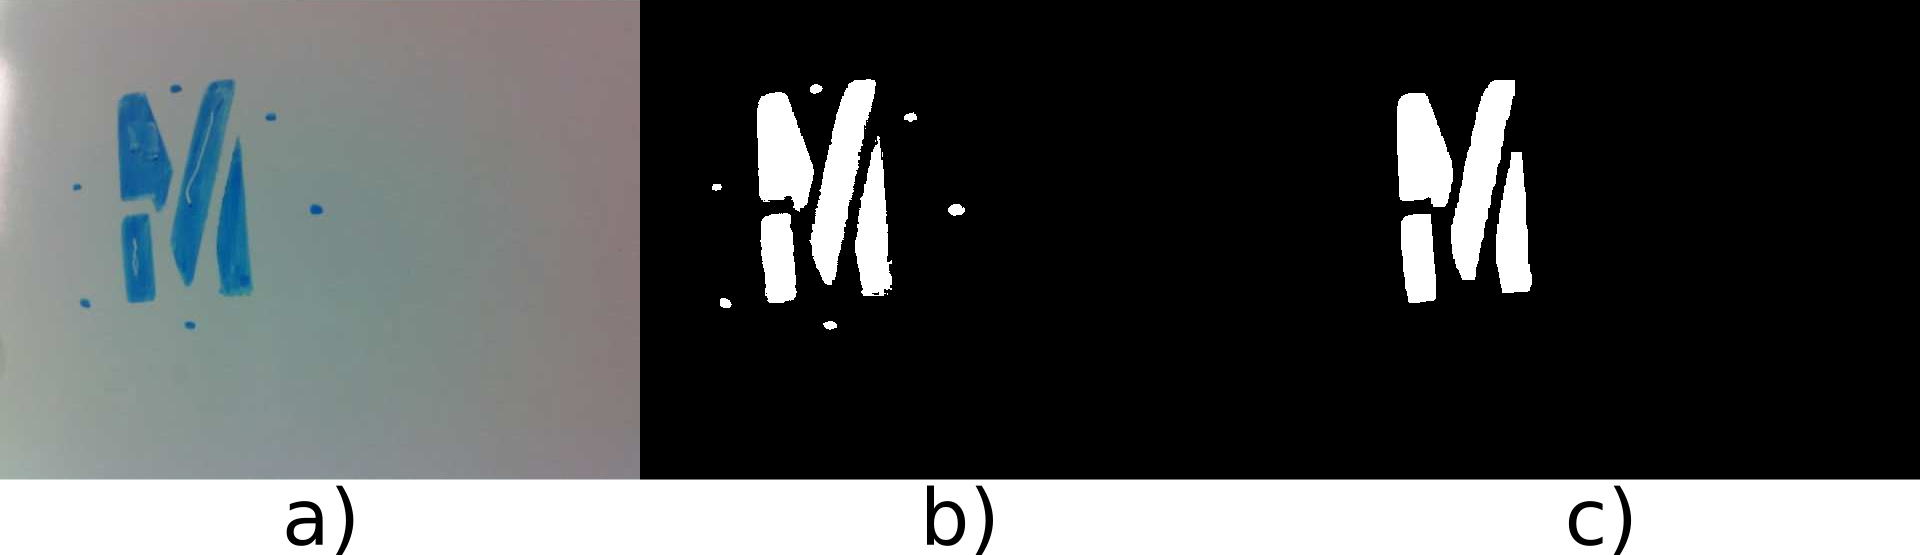
\includegraphics[width=10.5cm, keepaspectratio]{images/filtro.png}
      \caption{Filtro morfológico}
    \end{figure}
  \end{frame}
  %* --Nueva diapositiva
  \begin{frame}
    \frametitle{Obtención de centroide}
    \begin{figure}[h]
      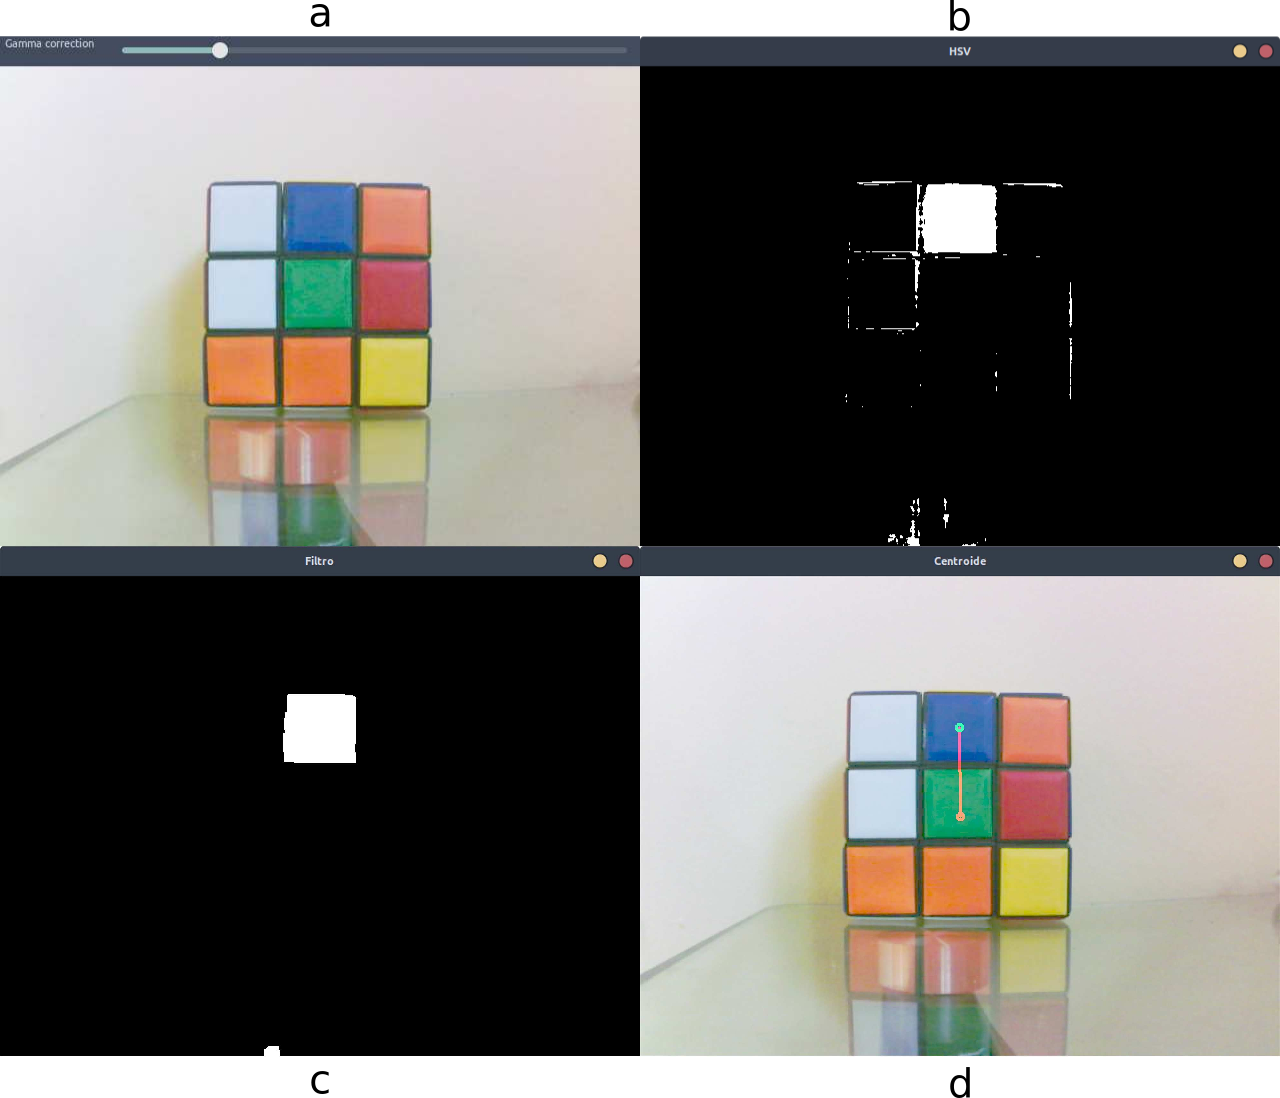
\includegraphics[height=5.5cm, keepaspectratio]{images/centroide.png}
      \caption{Filtro morfológico}
    \end{figure}
  \end{frame}
  % %* --Nueva diapositiva
  % \begin{frame}
  %   \frametitle{Obtención de centroide}
  %   \begin{figure}[h]
  %     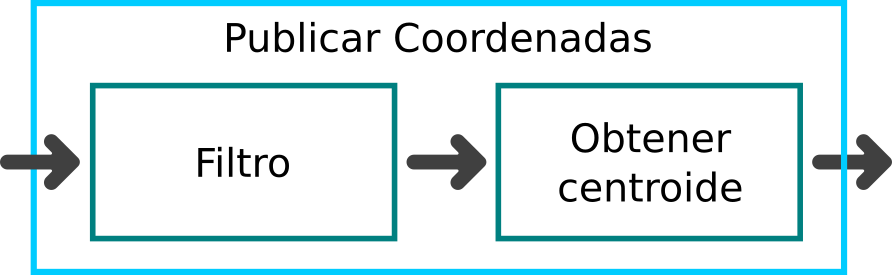
\includegraphics[width=10.5cm, keepaspectratio]{images/flowchart3.png}
  %   \end{figure}
  % \end{frame}
  % %* --Nueva diapositiva
  % \begin{frame}
  %   \frametitle{Visión}
  %   \begin{figure}[h]
  %     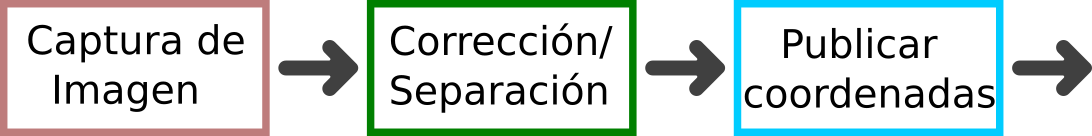
\includegraphics[width=10.5cm, keepaspectratio]{images/flowchart4.png}
  %   \end{figure}
  % \end{frame}
  

  %* --Nueva diapositiva
  \begin{frame}
    \frametitle{Control}
    \begin{itemize}
      \item La idea principal del sistema de control es la de encontrar una función de
      entrada $u(t)$ tal que la función de salida $x(t)$ siga la salida deseada $x^{des}(t)$
    \end{itemize}
    \begin{equation}
      e(t) = x^{des}(t) - x(t)
    \end{equation}
    \begin{equation}
      u(t) = k_i \int e(t) + k_p e(t)
    \end{equation}
    \begin{itemize}
      \item Coordenada Y -\textgreater Pitch
      \item Coordenada X -\textgreater Yaw
    \end{itemize}
  \end{frame}
  %* --Nueva diapositiva
  \begin{frame}
    \frametitle{Diseño de controlador}
    \begin{itemize}
      \item \textbf{Pitch} 
    \end{itemize}
    \begin{equation}
      J_{ay}\dot{q} = T_y 
    \end{equation}
    \begin{itemize}
      \item \textbf{Yaw}
    \end{itemize}
    \begin{equation}
      J_k\dot{r}_k = T_z
    \end{equation}
  \end{frame}
  %* --Nueva diapositiva
  \begin{frame}
    \frametitle{Diseño de controlador}
    \begin{figure}
      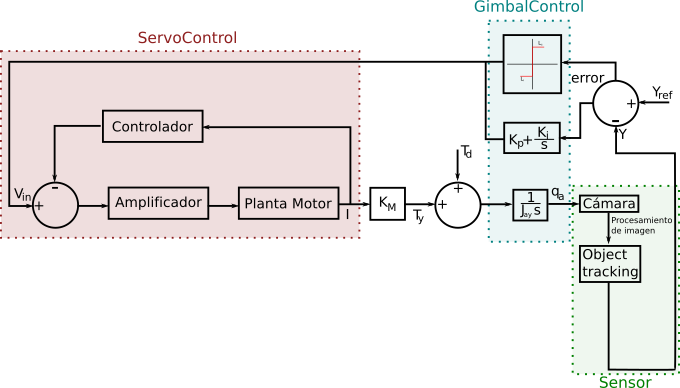
\includegraphics[width=10.5cm, keepaspectratio]{images/lazo-control-pitch.png}
    \end{figure}
  \end{frame}
  %* --Nueva diapositiva
  \begin{frame}
    \frametitle{Diseño de controlador}
    \begin{itemize}
      \item Control Proporcional Integral
      \item Asignación de Polos
    \end{itemize}
    \begin{equation}
      G(s) = \frac{1}{0.002s + 1}
    \end{equation}
    \begin{equation}
      C(s) = K_p(1 + \frac{1}{T_is})
    \end{equation}
    \begin{itemize}
      \item Aplicando lazo cerrado de (5) y (6), obtenemos la ecuación característica
    \end{itemize}
    \begin{equation}
      E.C_1 = s^2 + 500K_ps + \frac{500K_p}{T_i}
    \end{equation}
  \end{frame}
  %* --Nueva diapositiva
  \begin{frame}
    \frametitle{Diseño de controlador}
    \begin{itemize}
      \item Tiempo de asentamiento = 0.2s
      \item Porcentaje de error en 2\%
      \item Pico Máximo menor al 10\%
    \end{itemize}
    \begin{equation}
      G_d(s) = \frac{1086}{s^2+60s+1086}
    \end{equation}
    \begin{equation}
      E.C_2 = s^2 +60s + 1086 = s^2 + \alpha_1s + \alpha_2
    \end{equation}
    \begin{itemize}
      \item Igualamos $E.C_1$ con $E.C_2$ 
    \end{itemize}
    \begin{equation}
      500k_p = \alpha_1
    \end{equation}
    \begin{equation}
      \frac{500K_p}{T_i} = \alpha_2
    \end{equation}
  \end{frame}
  %* --Nueva diapositiva
  \begin{frame}
    \frametitle{Diseño de controlador}
    \begin{itemize}
      \item Control resultante
    \end{itemize}
    \begin{equation}
      C(s) = 0.118 + (1 + \frac{1}{0.054s})
    \end{equation}
    \begin{figure}
      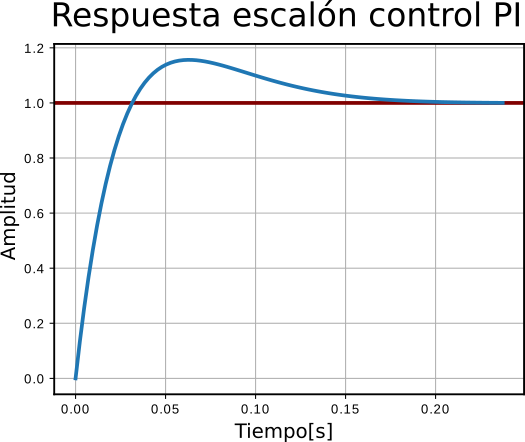
\includegraphics[height=4.1cm, keepaspectratio]{images/escalon-pitch.png}
      \caption{Respuesta a impulso escalón}
    \end{figure}
  \end{frame}
  %* --Nueva diapositiva
  \begin{frame}
    \frametitle{Diseño de controlador}
    \begin{multicols}{2}
      \begin{itemize}
        \item \textbf{Yaw}
      \end{itemize}
      \begin{equation} \nonumber
        G(s) = \frac{1}{0.008s + 1}
      \end{equation}
      \begin{equation}\nonumber
        C(s) = 0.312 + (1 + \frac{1}{0.08s})
      \end{equation}
      \begin{figure}
        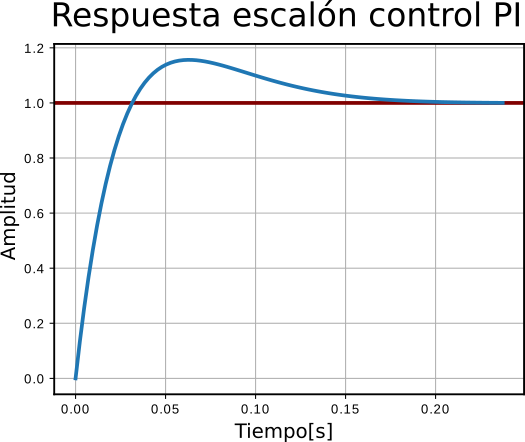
\includegraphics[width = 5.2cm, keepaspectratio]{images/escalon-yaw.png}
        \caption{Respuesta a impulso escalón}
      \end{figure}          
    \end{multicols}
  \end{frame}
  %* --Nueva diapositiva
  \begin{frame}
    \frametitle{Arquitectura}
    \begin{figure}
      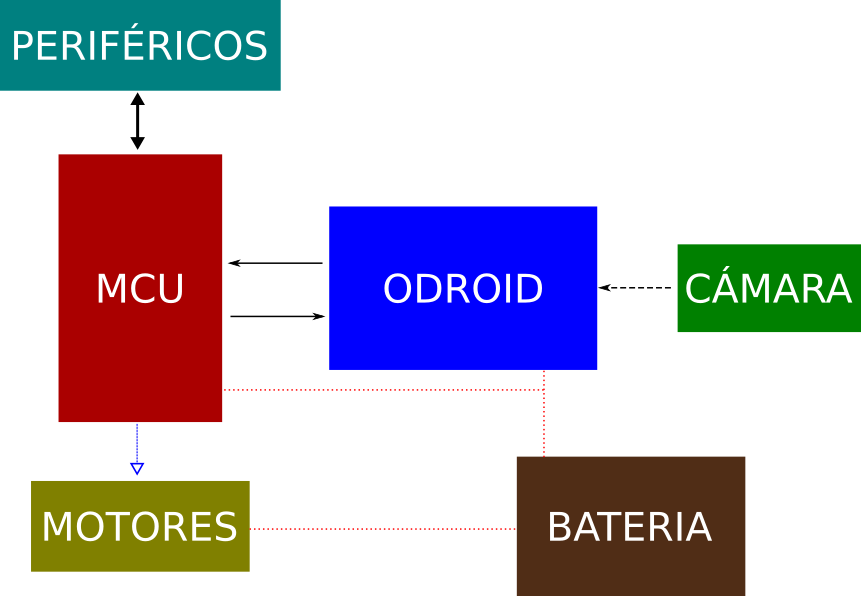
\includegraphics[height=5cm, keepaspectratio]{images/arquitectura.png}
      \caption{Arquitectura propuesta para el sistema}
    \end{figure}
  \end{frame}
  %* --Nueva diapositiva
  \begin{frame}
    \frametitle{Sistema Mecánico}
    \begin{figure}
      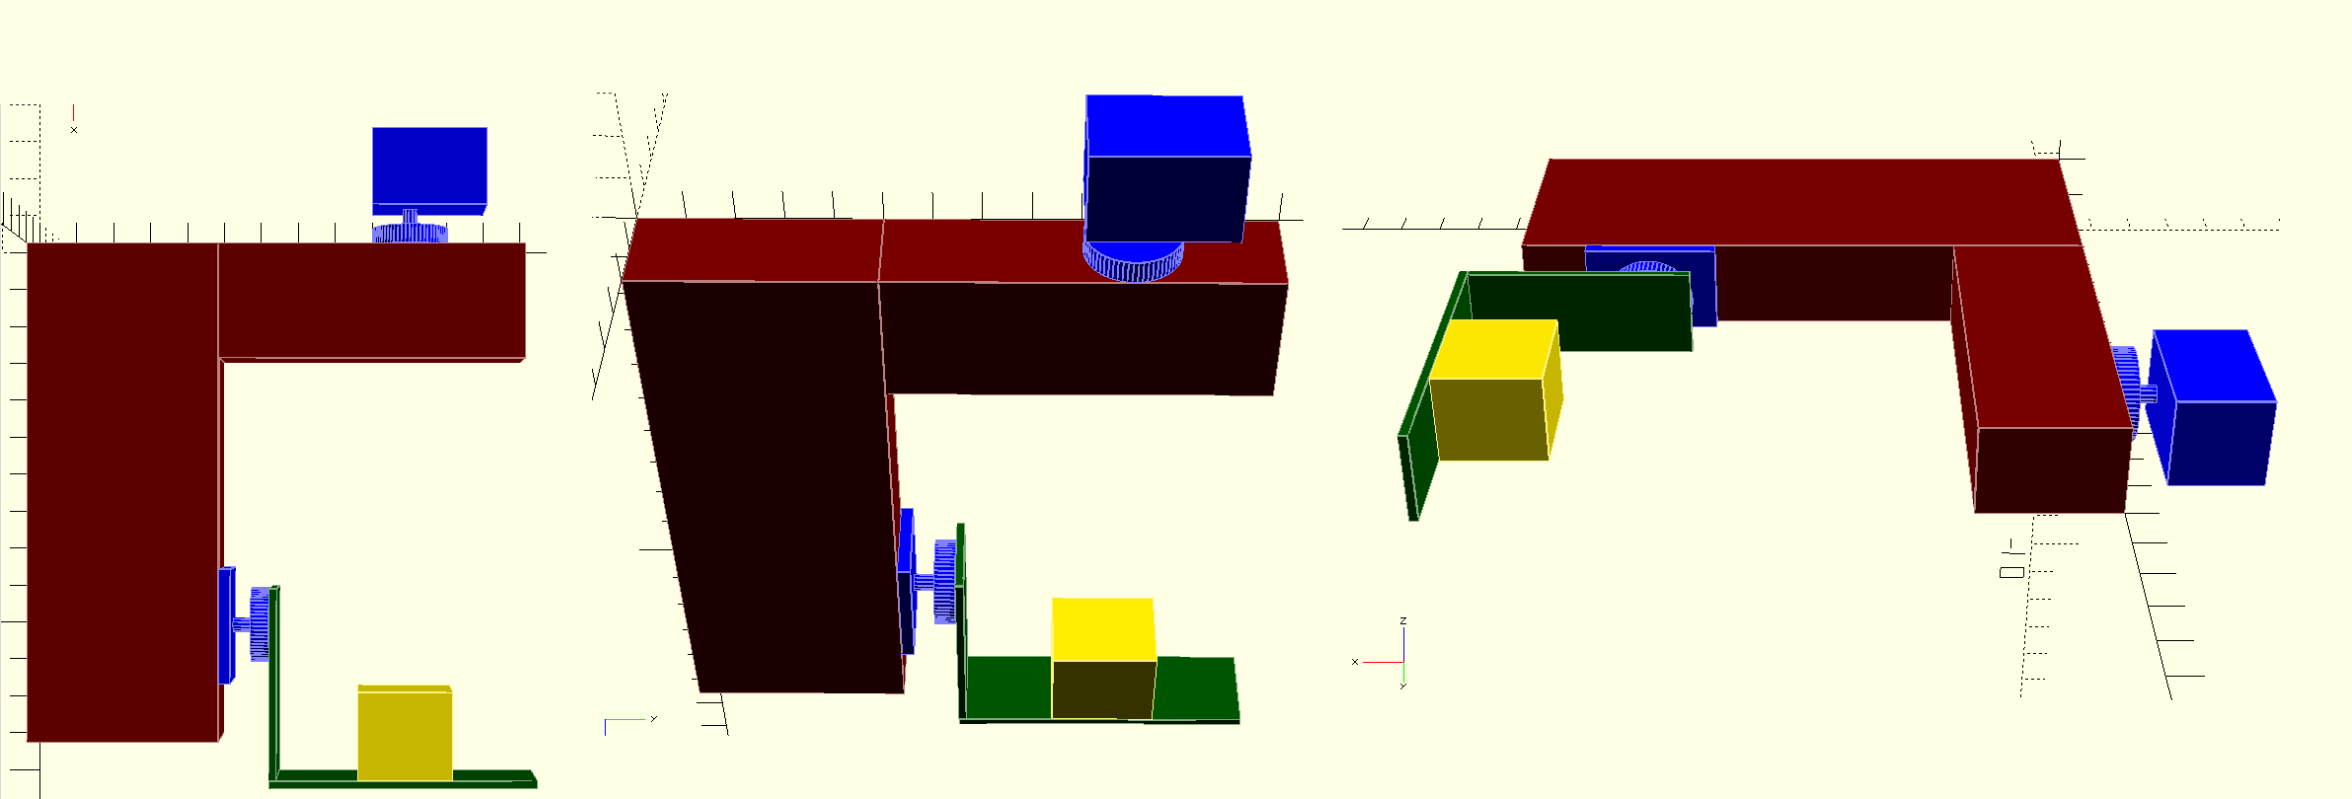
\includegraphics[width=10cm, keepaspectratio]{images/cad.png}
      \caption{CAD sistema mecánico}
    \end{figure}
  \end{frame}
  %* --Nueva diapositiva
  \begin{frame}
    \frametitle{Sistema Mecánico}
    \begin{figure}
      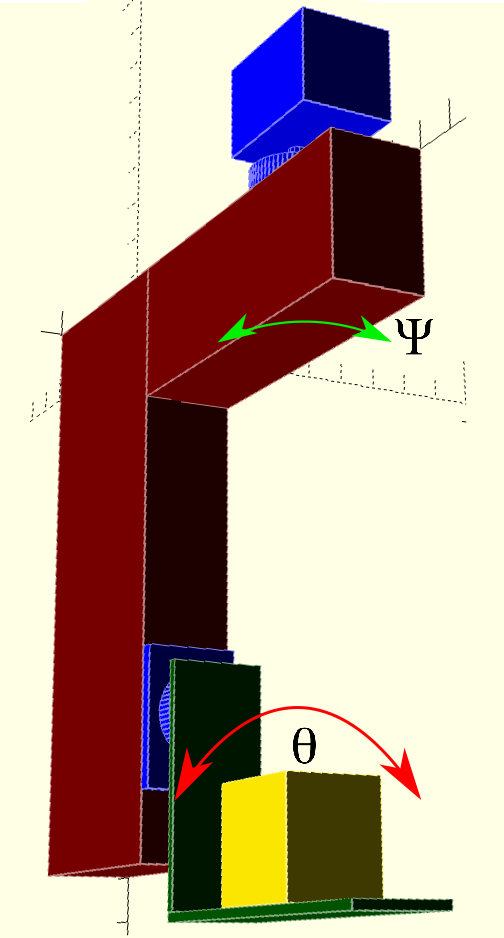
\includegraphics[height=5cm, keepaspectratio]{images/cad-2.png}
      \caption{CAD sistema mecánico}
    \end{figure}
  \end{frame}
  %* --Nueva diapositiva
  \begin{frame}
    \frametitle{Sistema Mecánico}
    \begin{figure}
      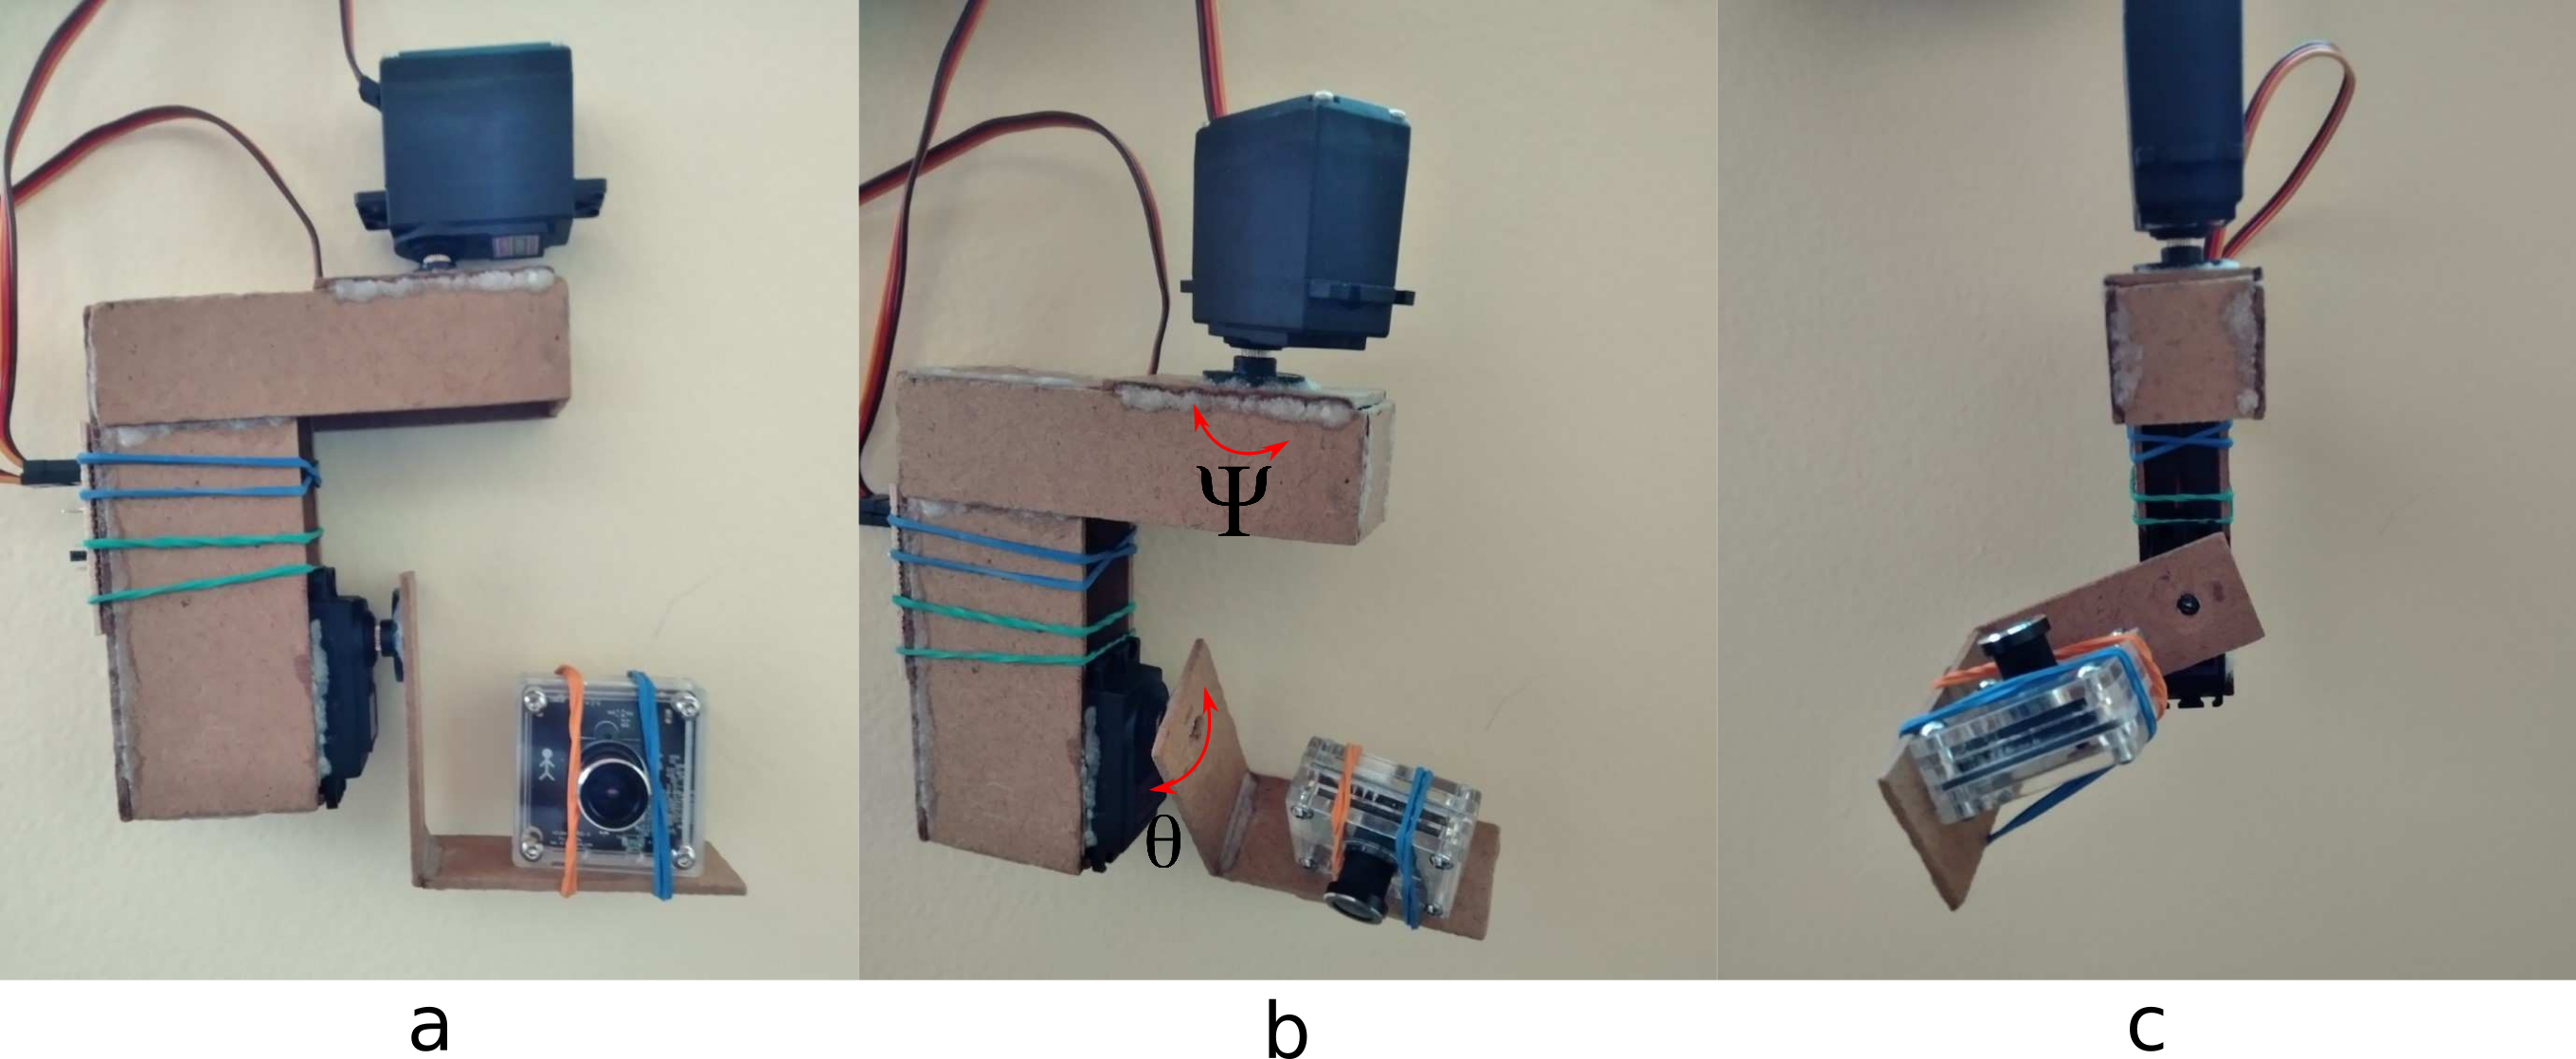
\includegraphics[width=10cm, keepaspectratio]{images/prototipo.png}
      \caption{Prototipo}
    \end{figure}
  \end{frame}


% !=============== RESULTADOS ===============
  \section{Resultados Finales}
  %* --Nueva diapositiva
  \begin{frame}
    \frametitle{Sintonización Pitch}
    \begin{figure}
      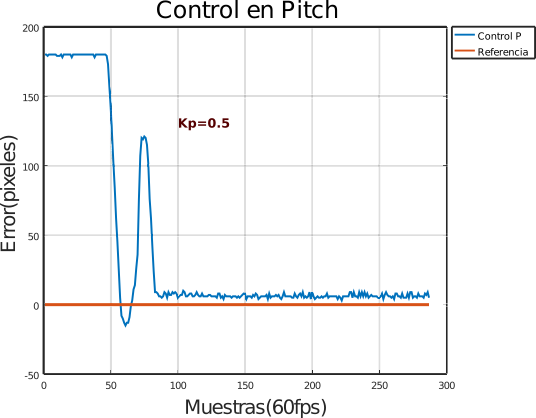
\includegraphics[height=6cm, keepaspectratio]{images/Sintonizacion-pitch.png}
      % \caption{Sintonizar Kp}
    \end{figure}
  \end{frame}
  %* --Nueva diapositiva
  \begin{frame}
    \frametitle{Sintonización Pitch}
    \begin{figure}
      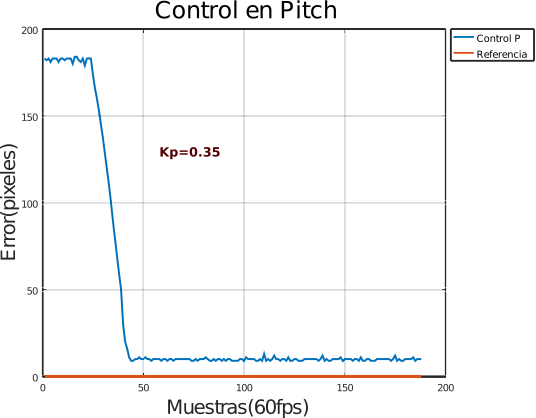
\includegraphics[height=6cm, keepaspectratio]{images/Sintonizacion-pitch1.png}
      % \caption{Sintonizar Kp}
    \end{figure}
  \end{frame}
  %* --Nueva diapositiva
  \begin{frame}
    \frametitle{Sintonización Pitch}
    \begin{figure}
      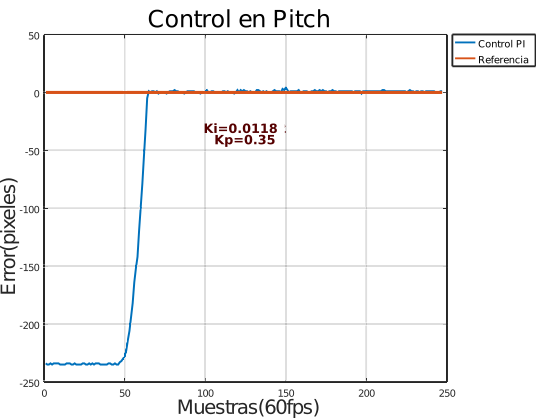
\includegraphics[height=6cm, keepaspectratio]{images/Sintonizacion-pitch2.png}
      % \caption{Sintonizar Kp}
    \end{figure}
  \end{frame}
  %* --Nueva diapositiva
  \begin{frame}
    \frametitle{Sintonización Yaw}
    \begin{figure}
      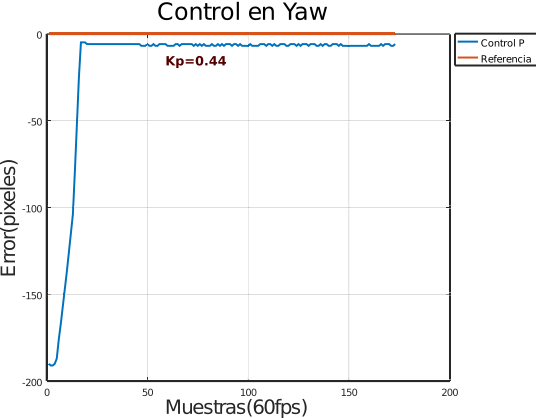
\includegraphics[height=6cm, keepaspectratio]{images/Sintonizacion-Yaw.png}
      % \caption{Sintonizar Kp}
    \end{figure}
  \end{frame}
  %* --Nueva diapositiva
  \begin{frame}
    \frametitle{Sintonización Yaw}
    \begin{figure}
      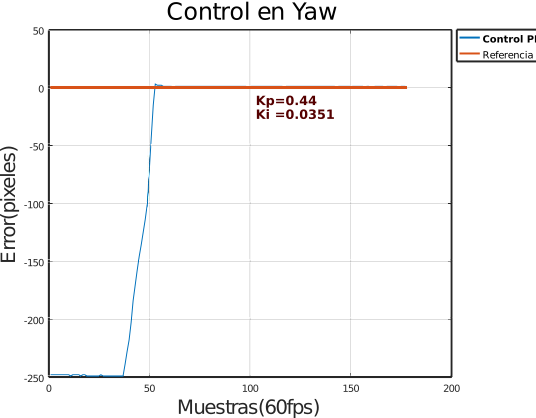
\includegraphics[height=6cm, keepaspectratio]{images/Sintonizacion-Yaw1.png}
      % \caption{Sintonizar Kp}
    \end{figure}
  \end{frame}
 

% !=============== CIERRE ===============
  \section{Cierre}
  %* --Nueva diapositiva
  \begin{frame}
    \frametitle{Futuros Trabajos}
    \begin{itemize}
      \item Implementación en drone.
      \item Agregar sensor de luminosidad.
      \item Cambiar a motores brushless.
      \item Diseñar control de velocidad-posición.
      \item Mejorar el diseño mecánico.
    \end{itemize}
  \end{frame}

\end{document}
